\documentclass[a4paper, 11pt]{scrartcl}

%\usepackage[a4paper, total={6in, 9in}]{geometry}

%========================================== Dokumentinformationen ===================================================

\title{Squad Maprotagenerator 2.0}
\subtitle{Für politische Entscheindungsträger}
\author{timbow, fletschoa, kappakay}

\usepackage[dvipsnames]{xcolor}

\usepackage[
	pdftitle={Squad Maprotagenerator 2.0},
	pdfsubject={},
	pdfauthor={timbow, fletschoa, kappakay},
	pdfkeywords={}
	pdftex=true, 
	colorlinks=true,
 	breaklinks=true,
	citecolor=blue,
	linkcolor=black,	
	menucolor=black,	
	urlcolor=blue
]{hyperref}

%========================================== Klassen ===================================================
\usepackage{hyperref}               % Hyperlinks zwischen Chaptern und TOC
\usepackage[backend=bibtex,language=german,style=ieee]{biblatex}
\usepackage{todonotes}              % Setzt Notes im fertigen PDF
\usepackage{amsmath,amssymb}        % basic Math package
\usepackage[german]{babel}
\usepackage{graphicx, subfigure}    % Bild-/file inputs
\usepackage{tikz}                   % notwendig für tikz-zeichnen in Latex selbst

\usepackage{fancybox}               % Zitate-box
\usepackage{yfonts}                 % Alt-deutsche Buchstaben
\usepackage{forest}                 % Baumdiagramme, alternative zu Tikz
\graphicspath{{img/}}

\newenvironment{boxedlaw}[1]
  {\begin{Sbox}\begin{minipage}{#1}\centering}
  {\end{minipage}\end{Sbox}\begin{center}\shadowbox{\TheSbox}\end{center}}

%include bib data
\bibliography{bibtex.bib}

\begin{document}
    
    \maketitle
    \newpage
    \tableofcontents
    \newpage

    \begin{boxedlaw}{10cm}
        \textswab{Memory Colonel, der du bist in GooseBay, geheiligt werde dein Name.}\\
        \textswab{Deine Rota komme.}\\
        \textswab{Deine locktime geschehe.}\\
        \textswab{Unser täglich Squad gib und heute.}\\
        \textswab{Und vergib uns unser Minen legen, wie auch wir vergeben unseren snipern}\\
        \textswab{Und führe uns nicht in Versuchung, sondern erlöse uns von Tallil}\\
        \textswab{Denn dein ist die Rota und Biome und die Abwechslung in Ewigkeit.}\\
        \textswab{Amen}\\\

        - \textit{Das Maprota Gebet}
    \end{boxedlaw}

    \newpage
    \listoffigures
    \label{sec:abkuerzungverzeichnis}
    %\addchap{Abkürzungverzeichnis}
    \addcontentsline{toc}{section}{Abbildungsverzeichnis}
    \newpage
    %\listoftables
    %\addcontentsline{toc}{chapter}{Tabellenverzeichnis}
    %\newpage

    \section{Einleitung}
        
        Der gemeine Squad Spieler mag nach der Sammlung an einiger Erfahrung gemerkt haben, dass eine abwechslungsreiche Rotation von Layern (Maprota)
        die Qualität das Spieles deutlich verbessert. So fiel uns in der Vergangenheit auf, dass auf dem We $\heartsuit$ Squad Discord sich immer wieder 
        Spieler über die Maprota beschwert haben. Anfangs beschwerten wir uns auch, bis wir uns das Ziel gesetzt haben, ein Programm 
        für die Generierung einer besseren Maprota zu schreiben, bevor wir uns wieder beschweren. 
        Die Ziele, für das Projekt, waren schnell aufgestellt und das Problem scheint im ersten Moment einfach lösbar zu sein.
        Wir können euch nach 2 Monaten Entwicklungszeit aber sagen es ist definitiv nicht einfach! Es wäre einfacher gewesen sich weiterhin zu beschweren.
        Die Lösung, die wir für eine bessere Maprota gefunden haben, möchten wir hier vorstellen.  

        \subsection{Problemdarstellung}
            Aus den historischen Debatten über die Maprota wurde versucht, die Hauptprobleme hervorzuheben und werden im folgenden erklärt.

            Der Mapgenerator soll qualitativ hochwertige Maprotas generieren.
            Zur Klassifizierung werden wir nun zunächst Eckpunkte definieren welche die Qualität einer Rota bemessen sollen.

            Zunächst sollte sich eine Map nicht zu stark wiederholen.
            Des Weiteren gab es in der Community bedenken, welche sich damit beschäftigen, dass nicht zu ähnliche Maps zu kurz hintereinander gespielt werden sollten. 
            Ein Beispiel für letzteres wäre die Abfolge 
            \begin{equation*}
                \text{Sumari} \rightarrow \text{Logar Valley} \rightarrow \text{Fallujah}.
            \end{equation*}
            Hier würden direkt nacheinander folgend drei relativ ähnliche Maps gezogen werden. 
            Der Charakter dieser Maps wird im wesentlichen über die Eigenschaften \glqq{}Wüste\grqq{}, \glqq{}Stadt\grqq{}, \glqq{}Infanterie lastig/klein\grqq{} der Map definiert.
            Eine gute Rota sollte solche Map-Ketten vermeiden.

            Ein weiterer wichtiger Punkt ist die Vermeidung von Mustern in der Rota. 
            Das bedeutet, dass die generierten Rotas nicht deterministisch verteilt, sondern aus zufälligem Ziehen entstehen sollen.
            
            Das seit einiger Zeit bestehende Layervote-System muss direkten Einfluss auf die Rota haben um die Verteilung den Wünschen der Community anzupassen.
        \newpage
        \subsection{Ziel}
        \label{sub:Ziele}
            Zusammenfassend werden wir im folgenden die Qualität der Maprota an folgenden Eigenschaften messen:
            \begin{itemize}
                \item Ähnlichkeit der gezogenen Maps in kurzem Zeitraum
                \item Wiederholung der selben Map in kurzem Zeitraum
                \item Keine Muster/Nicht-deterministische Verteilung 
                \item Layervotes müssen direkten Einfluss haben 
            \end{itemize}

            Der in diesem Dokument beschriebene Algorithmus soll alle vier genannten Eigenschaften so gut wie möglich Erfüllen.
            Kurz gesagt ist das Ziel des Maprota Generators:\\\
            \glqq{}Ein probabilistisches System dessen globale Verteilung durch Mapvotes gegeben ist und lokal Wiederholung ähnlicher Maps vermeidet.\grqq{}
            Anders ausgedrückt:\\
            Das System sollte global einer Verteilung folgen welche die Map/Layervotes wiederspiegeln und lokal eine gewisse Varianz unter den Mapcharakteristiken hervorruft.

            Im weiteren Verlauf wird ein Algorithmus präsentiert, welcher alle oben genannten Aspekte so gut wie möglich abdeckt. 
            Es sei aber darauf hingewiesen, dass nicht alle Punkte gleichzeitig perfekt umgesetzt werden können aufgrund kritischer Eigenschaften des Systems und der gesetzen Nebenbedingungen.
            Darauf wird im Folgenden noch näher eingegangen.

    
    \section{Theoretische Grundlagen}
    Eine Maprota besteht aus einer festen Anzahl an Layern mit verschiedenen Gamemodes. 
    Zu beginn der Abfolge wird noch eine feste Anzahl an Seedmaps gelistet welche jedoch für die Mapverteilung des Rota-Generators statistisch irrelevant sind.
    Die folgenden Abschnitte beschäftigen sich mit den benutzten mathematischen Modellen und definiert alle notwendigen Objekte.
    Der genaue Aufbau des Generators ist im nächsten Kapitel zu finden.
    \subsection{Wahrscheinlichkeitsmaß}
        Wie im vorherigen Kapitel dargelegt ist das Ziel eine Mapverteilung zu bekommen welche einer vorgegebenen Verteilung folgt und lokal ein ''Gedächtnis'' besitzt.
        Die vorgegebene Verteilung wird aus den Layervotes generiert, kann aber prinzipiell jede beliebge diskrete Wahrscheinlichkeitsverteilung 
        \begin{equation}
            p_{M,\text{fi}}(m) := \sum_{i=1}^N \mathbb{P}(M=m)
        \end{equation}
        sein, wobei $\mathbb{P}(M=m)$ die Wahrscheinlichkeit ist dass die Map $m$ gezogen wird, repräsentiert durch die Zufallsvariable $X$.
        Das ''Gedächtnis'' wird im folgenden als \textbf{Memory Kernel} bezeichnet.
        Um die obige Verteilung $p_{x,\text{fi}}(x)$ zu realisieren werden mehrere intere Weights verwendet um ein auf System zu repräsentieren welche sich aus mehreren Stufen des ''Ziehens'' eines Gamemodes/Map/Layers zusammensetzt.
        Die Maprota wird dann durch folgende multivariate Verteilung modelliert
        \begin{align}
            p_{G,M,L}(g,m,l)    &= P(G=g, M=m, L=l) \\
                                &= P(G=g)\cdot P(M=m|G=g) \cdot P(L=l|G=g, M=m)
        \end{align}
        wobei $G,M,L$ die Zufallsvariablen "Gamemode", "Map" und "Layer" sind und $P(A|B)$ die bedingte Wahrscheinlichkeit für das Ereignis $A$ unter der Nebenbedingungen das zuvor $B$ eingetreten ist.
        Die Wahrscheinlichkeit für ein Layer wie "Yehorivka RAAS v3" ist damit gegeben durch 
        \begin{equation*}
            \mathbb{P}(\text{''Yehorivka RAASv3''}) = p_{G,M,L}(\text{''RAAS'', ''Yehorivka'', ''RAASv3''})
        \end{equation*}
        Das Ziel ist die einzelnen bedingten Wahrscheinlichkeiten so zu wählen, dass wir die Übereinstimmung
        \begin{equation}
            p_{M,\text{fi}}(m) \equiv \sum_{g,l}p_{G,M,L}(g,m,l)
        \end{equation}
        haben, oder zumindest in einer Umgebung dieser Lösung sind definiert durch 
        \begin{equation}
            \sum_m |p_{M,\text{fi}}(m)-\sum_{g,l}p_{G,M,L}(g,m,l)|<\epsilon  
        \end{equation}
        für $\epsilon>0$ aber $\epsilon << 1$.
        \subsubsection{Mode Wahrscheinlichkeiten}
            Die Modewahrscheinlichkeiten definiert durch $p_G(g)=\mathbb{P}(G=g)$ werden \textit{a priori} gesetzt da das Ziehen des Gamemodes der erste Schritt in der Rota-Generierung ist.
            Prinzipiell kann diese von Hand gesetzt werden. 
        \subsubsection{Map Wahrscheinlichkeiten}
            Die Mapwahrscheinlichkeiten              
        \subsubsection{Verteilungsfunktionen}
        Die Gamemode-Wahrscheinlichkeiten werden von Hand gesetzt. 
        Sollte eine Map $m$ nicht im Gamemode $g$ vorhanden sein, so ist die bedingte Wahrscheinlichkeit $P(M=m|G=g) = 0$. 
        Falls die Map vorhanden ist so wird die Wahrscheinlichkeit zum ziehen der Map errechnet aus den Mapvotes verglichen mit den anderen Maps und der Ähnlichkeit zu den zuvor gezogenen Maps.
        Wenn eine Map $m$ gezogen wurde wird ein Layer $l$ nach der Verteilung der Mapvotes der in frage kommenden Layern gezogen. 
        Es ist dann gegeben durch 
        \begin{equation}
            \mathbb{P}(\text{''Layer A''}) = \frac{S(v_i)}{\mathcal{N}}
        \end{equation}
    \subsection{Oberflächliches Model - Baumdiagramm}
        Die statistische Natur der Maprota kann als "Würfeln" verschiedener Layer verstanden werden. 
        Der Algorithmus setzt sich aus zwei Schichten zusammen: Zunächst wird ein Modus gezogen z.b. "Invasion". 
        Die Wahrscheinlichkeit dass ein Modus gezogen wird ist \textit{a priori} gesetzt und wird als externe Größe in den Generator gegeben.
        Nach ziehen des Modus folgt nun die Auswahl der Map. 
        Die Wahrscheinlichkeit das eine Map gezogen wird hängt von den Mapvotes ab und weiteren internen Parametern. 

        \begin{figure}
            \begin{forest}
                for tree={
                  math content,
                  if n=0{coordinate}{circle,draw=black,fill=red!10},
                  grow=0,
                  l=3cm
                }
                [
                 [\overline{A},edge label={node[midway,below=2pt]{$q_1$}}
                  [\overline{D},edge label={node[midway,below]{$p_{21}$}}
                   [\overline{L},edge label={node[midway,below]{$l_{211}$}}]
                   [L,edge label={node[midway,below]{$l_{212}$}}]
                  ]
                  [D,edge label={node[midway,above]{$p_{22}$}}] 
                 ]
                 [A,edge label={node[midway,above=2pt]{$q_2$}}
                  [\overline{D},edge label={node[midway,below]{$p_{11}$}}]
                  [D,edge label={node[midway,above]{$p_{12}$}}] 
                 ]
                ]
            \end{forest}
        \caption{Baumdiagramm zur Zusammensetzung der Mapwahrscheinlichkeiten. 
        Die Wahrscheinlichkeiten, einen Mode zu ziehen, sind $q_1$ und $q_2$ für Mode $1$ und $2$ repsektiv.
        Die Wahrscheinlichkeit, eine Map unter gegebenen Modus zu ziehen, ist gegeben durch $p_{ij}$, d.h. $p_{12}$ ist die bedingte Wahrscheinlichkeit dass Map $2$ gezogen wird wenn vorher Mode $1$ gezogen wurde.}
        \end{figure}
    \subsection{Mapvoteweights}
        Zur Realisierung der Verteilung werden Mapwahrscheinlichkeiten benötigt. 
        Diese werden aus den Layervotes wie folgt gewonnen:\\
        Sei $\mathcal{M}$ die Menge aller Maps. 
        Desweiteren sei $v\in\mathbb{Z}$ die Anzahl an Votes eines Layers.
        Dann wird das Weight für ein $m\in \mathcal{M}$ berechnet nach 
        \begin{align*}
            \mu_i &= \frac{1}{N}\sum_{i=1}^N v_i\\
            w_i &= \exp\left(-(\mu_i-v_i)^2\right)\\
            \bar{w}_i &= \frac{w_i}{\sum_i w_i}\\
            \bar{v}_\text{map} &= \sum_{i=1}^N\bar{w}_i\cdot v_i
        \end{align*}
        Der Mapvote einer Map für einen Modus errechnet sich als das gewichtete arithmetische Mittel aller Votes im selben Modes der Map.
        Das Gewicht eines Votes ist so definiert dass Vote-summen fern des Erwartungswertes weniger stark ins Gewicht fallen.
        Damit soll verhindert werden, dass einzelne "Ausreißer" die globale Map-Bewertung zu sehr herunterziehen.
        \begin{figure}[htbp]
            \centering
            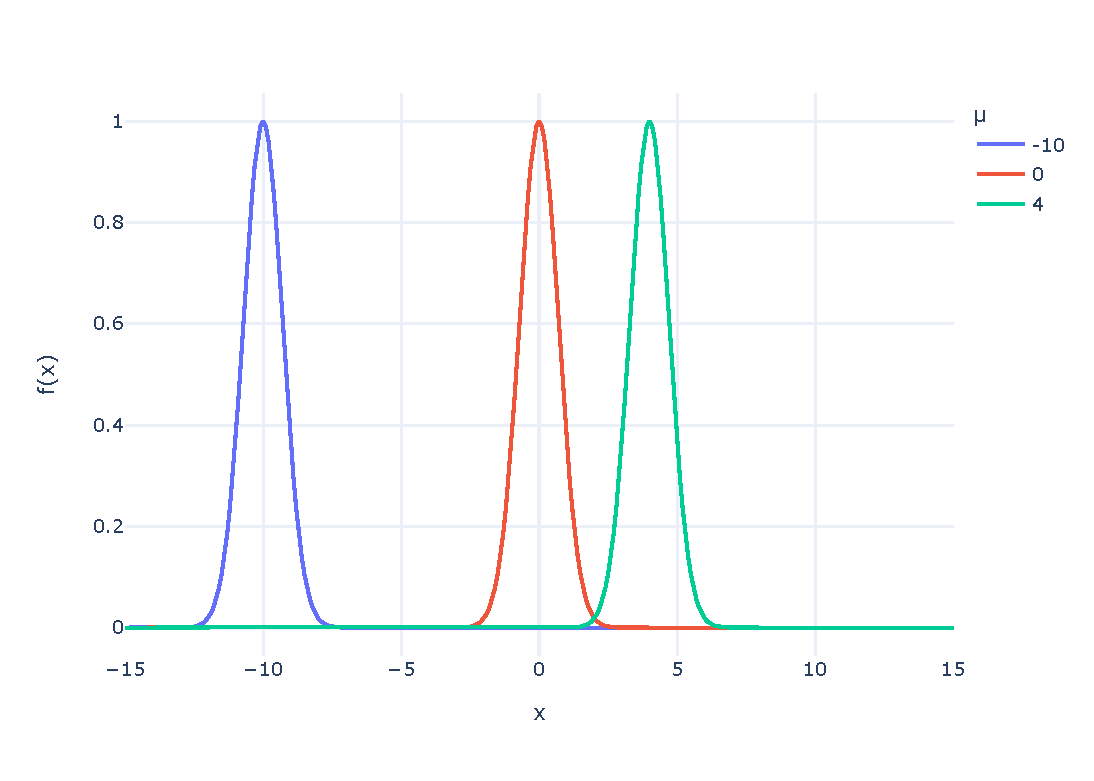
\includegraphics[width=0.85\textwidth]{plot_gaus.pdf}
            \caption{Die Weightfunktion $w_i=f(x)$ geplottet für verschiedene Erwartungswerte.
            Je weiter die Vote-Anzahl vom Mittelwert entfernt ist desto kleiner ist das errechnete Weight und das Layer wird somit stärker bestraft und als ''Ausreißer'' gewertet.}
        \end{figure}
        \subsection{Die Kugel}
    % was muss hier erklärt werden
    % was ist eine rota
    % Überblick aus dem Game, was sind modes was sind map was sind layer, was sind biome 
    % kleine einführung in mathe 
    % was ist eine gute und eine schlechte rota
    Um den ''Map-Charakter'' verschiedener Maps zu vergleichen, werden zunächst verschiedene Charakteristiken definiert wie zum Beispiel ''Wüste'' oder ''Stadt''.
    Jede Map wird ein Anteil an jeder Charakteristik zwischen $0$ und $1$ zugeschrieben, was respektiv dafür steht dass die Eigenschaft gar nicht oder absolut zutrifft für die Map.
    Zum Beispiel würde eine Map mit ''Winter-Setting'' welche nur aus Gebirge besteht in jeder der beiden Eigenschaften den Wert $1$ erhalten. 
    Die Bewertung der einzelnen Maps ist jedoch subjektiv.
    Um den Vergleich zweier Maps zu schaffen wird das System wiefolgt repräsentiert:
    Zu jeder Map $m$ existiert ein ''Biom-Vektor'' $\vec{b} = (b_1,.....,b_n)^T$. 
    Hier stehen die Vektorkomponenten $b_i$ für die obengenannte Zuordnung der entsprechenden Charakteristik und $n$ ist die Anzahl der Vorhandenen Charakteristiken.
    Anschließend wird der Vektor normiert sodas $|\vec{b}|=1$.
    Dadurch wird genau genommen wird der Raum aller Maps-Charakteristiken definiert durch die Hyperfläche
    \begin{equation*}
        \mathcal{L} = \{\vec{x}\in\mathbb{R}^n ||\vec{x}|=1 \land 0\leq x_i \leq \smash{\frac{\pi}{2}} \quad \forall i\in\{1...n\}\}
    \end{equation*}
    Das bedeutet, dass die Maps durch Punkte auf dem Rand der $1/2^n$-tel Kugel beschrieben werden.

    Zwei Maps sind ''ähnlich'', sofern die Punkte nahe beieinander liegen, da in diesem fall die Vektorkomponenten fast alle gleich sind wodurch sich die beiden Vektoren lediglich um einen kleinen Winkel unterscheiden.
    Da die Vektoren normiert sind, entspricht dies einer kleinen Distanz auf der Kugeloberfläche.
    Die Distanz $l$ zweier Punkte auf der Kugel wird im Mapweight verrechnet und ist gegeben durch 
    \begin{equation}
        d = 2\arccos(\vec{a}\cdot\vec{b})
    \end{equation}
    für zwei Map-Charakteristiken $\vec{a}$ und $\vec{b}$, wobei $\cdot$ das innere Produkt (''Skalar Produkt'') bezeichnet. 
    \subsection{Mapweight}
    Das Weight errechnet sich als Produkt aus einem ''Distanz-Weight'' und einem ''Mapvote-Weight''. 
    \begin{equation}
        w_m(m,d,v) = \frac{1}{\mathcal{N}}w_d(d,m)w_v(v,m)
    \end{equation}
    wobei $\mathcal{N}$ das Produkt-Weight normiert sodass $\sum_m w_m = 1$.
    \subsubsection{Distanzweight}
        Das Distanzweight ist eine allgemeine stückweise stetige Funktion definiert durch
        \begin{equation}
            w_d : \mathbb{R}^+ \rightarrow \mathbb{R}^+, d \mapsto w_d(d),
        \end{equation}
        und der Nebenbedingung $w_d(d)\overset{d\rightarrow 0}{\longrightarrow}0$.
        In der momentanen Version ist die Funktion gegeben durch
        \begin{equation}
            w_d(d) = 1_{[0,d_\text{min}]}(d)
        \end{equation}
        mit $d_\text{min}\geq 0$ als Mindestdistanz. 
        Sollte eine Map näher als $d_\text{min}$ an einer zuvor gezogenen Map liegen ist das Distanzweight und damit das Mapweight $0$ und wird damit nicht gezogen. 
    \subsubsection{Mapvoteweight}
        Das Mapvoteweight wird aus dem Mapvote berechnet unter Nutzung einer Sigmoid funktion. 
        \begin{equation}
            w_v(v) = \frac{1}{1+\exp\left(-(av+b)\right)}
        \end{equation}
        wobei $v$ die Summe aller Layervotes eines Modus einer Maps ist und $a$ und $b$ zwei freie Parameter sind.
        Während $a$ die Steigung moduliert kann mit $b$ ein Offset erzeugt werden.
        Die Sigmoid funktion erlaubt es ein kontinuierliches weight zu definieren wodurch eine Map oder ein Layer nicht abrupt verschwindet sondern langsam ändert.
        \begin{figure}[htbp]
            \centering
            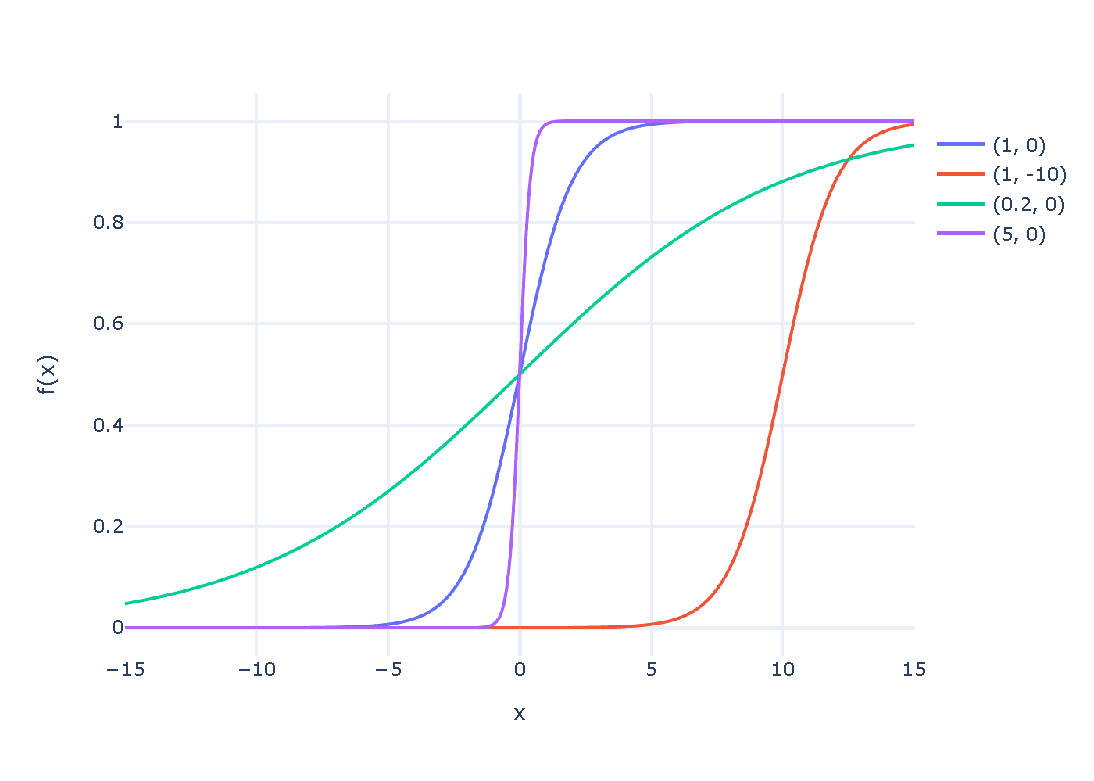
\includegraphics[width=0.85\textwidth]{plot_sigmoid.pdf}
            \caption{Die Sigmoidfunktion für mehrere Werte $a$ und $b$. 
                        Für $b=0$ ist für alle Werte $a$ $f(0)=1/2$.
                        Der Parameter $b$ dient als Offset.}
        \end{figure}
        \todo{sigmod abbildung nicht in text eingebunden}
    \subsection{Zusammenfassung}

    % was ist eine kugel und was meint tim damit 
    % wie werden die mapvotes ausgerechnet


    \section{Aufbau}
    Im Folgenden wird der Aufbau des Algoritmus näher beschrieben. 
    Nach einem kurzem Überblick werden die einzelnen Subsysteme detailiert erklärt.
    \subsection{Grundlegende Struktur}
    % oberflächliche Beschreibung des systems
    Die oberflächliche Struktur des Generators ist im unteren Flussdiagram dargestellt. 
    Für eine gegebene Anzahl an Layern in einer Rota wird für jedes Layer folgedne Routine ausgeführt:
    \begin{itemize}
        \item wähle einen Modus, gewichtet nach den Mode-Wahrscheinlichkeiten und dem Mode-Spacing
        \item für den gewählten Modus werden die validen Maps gefiltert
        \begin{itemize}
            \item zunächst wird geprüft welche Map im Modus repräsentiert ist
            \item aus den vorhanden Maps wird nach dem Distanz-Vote-Weight $w_m$ gewichtet eine Map gezogen
        \end{itemize}
        \item für die gezogene Map wird gewichtet nach dem Layerweight $w_l$ ein Layer gezogen
        \item die gezogenen Maps verbleiben für eine feste Maplänge im Memory-Kernel und sind damit für die nächsten Map Ziehungen nicht verfügbar
    \end{itemize}
    \subsection{Aufbau im Detail - Mode}
        Wie zuvor erwähnt gibt es zwei Faktoren die die Ziehung des Modus beeinflussen:
        \begin{itemize}
            \item [1.] die Modeweights die zuvor gesetzt wurden $w_g$ 
            \item [2.] das Modespacing
        \end{itemize}
        Desweiteren erlaubt der Generator eine Gruppierung der Modes in soganennte ''Pools''. 
        Es gibt immer einen sogenannten \textit{main}-Pool. 
        Ohne weitere Einstellungen ist erstmal jeder Modus der gespielt werden soll damit automatisch im Main-Pool enthalten. 
        Neben diesem können noch händisch weitere Pools definiert werden. 
        In der momentanen Fassung existieren drei Pools:
        \begin{itemize}
            \item \textbf{main}: Der zuvor erwähnte Standard-Pool, beinhaltet \textit{RAAS} und \textit{AAS}
            \item \textbf{intermediates}: Beinhaltet die Modi \textit{Invasion} und \textit{TC}
            \item \textbf{reste}: Beinhaltet \textit{Destruction} und \textit{Insurgency}
        \end{itemize}
        Das \textbf{Modespacing} sorgt nun dafür dass für eine gegebene Anzahl an Runden nur der Main-Pool gezogen werden darf.
        Mit anderen Worten kann durch das Modespacing eine Mindestzeit definiert werden in der es nur Main-Modi geben kann. 
        Sollte die Zeitspanne seit dem letzten nicht-main Modus größer sein als das Modespacing so wird mit den Pool und Mode-weights gewichtet ein Gamemode gewählt. 
        Hierbei wird erst der Pool ausgewählt und anschließend im Pool der Modus. 
        Es ist zu beachten dass dies dazu führen kann und wird, dass nicht direkt nach Ablauf des Modespacings ein andere Pool drankommen muss. 
        Das Design wurde mit Absicht so gewählt um repititive Modes zu verhindern.

    \subsection{Aufbau im Detail - Map}
    Jeder Map die im Modus enthalten ist wird ein Mapvoteweight $w_m$ und ein Distanzweight $w_d$ zugeordnet. 
    Aus dem Produktweight wird anschließend die Map gezogen. 
    Hier kommt noch hinzu dass die Distanzweights vom Memory-Kernel abhängen. 
    In der momentanen Implementierung bedeutet dies, dass eine Map welche in den letzten $k$ Runden gezogen wurde nicht nochmal dran kommen kann. 
    Effektiv heißt dies $w_d=0$ für diese Map. 
    Für den seltenen Fall dass keine Map verfügbar ist für einen Modus weil alle in Frage kommenden Maps zurzeit gesperrt sind wird der Modus in den sogenannten \textbf{Mode-Buffer} verlegt. 
    Dieser wird beim ziehen des nächsten Modus abgearbeitet. 
    Das bedeutet ein Modus wird "ge-queued" und kommt bei der nächst passenden Gelgenheit dran. 
    
    \subsection{Aufbau im Detail - Layer}
    Sobald eine Map ausgewählt wurde wird das Layer gewichtet nach dem Layerweights $w_l$ gezogen. 
    Diese hängen nur von den Mapvotes ab welche mit der vorher genannten Sigmoidfunktion moduliert werden. 
    \begin{figure}[htbp]
        \begin{tikzpicture}
            [scale=.8,auto=left,every node/.style={circle,fill=blue!20}]
            \node (n1) at (1,10) {Gorodok};
            \node (n2) at (4,8)  {Yehorivka};
            \node (n3) at (8,9)  {Blackcoast};
            \node (n4) at (11,8) {Skorpo};
            \node (n5) at (15,10) {Sumari};
            \node (n6) at (20,8)  {Logar};
            \node (n7) at (17,9)  {Fallujah};
            \foreach \from/\to in {n1/n2,n1/n3,n2/n3,n3/n4,n5/n6,n5/n7,n6/n7}
            \draw (\from) -- (\to);  
        \end{tikzpicture}
    \caption{Cluster}
    \end{figure}

    \section{Mapweights}

    \section{Ergebnisse}
    \subsection{Bewertung des Systems}
        Um den entstandenen Maprotagenerator bewerten zu können und den Grad der Qualität festellen zu können, 
        werden die Metriken aus Kapitel \ref{} \todo{ref} zur Hilfe genommen. Die Metriken sind für Squadmaprotas
        allgemeingültig und anhand dessen könnten sie miteinader verglichen werden. Es soll nicht unerwähnt bleiben,
        dass durch eine schlechte oder auch falsche Wahl der Einstellparameter das Maprotasystem leicht bis hin zu 
        sehr stark beeinträchtigen werden kann. Genaueres dazu ist unter \ref{s:grenzen_des_systems} nachzulesen.
        Daher ist bei diese Bewertung zu berücksichtigen, dass von uns wohl überlegte Einstellparameter festgelegt wurden
        und als Referenz für Änderungen herangezogen werden sollten.
        Das Wählen passender Einstellparameter kann in User manual nachgelesen werden.
   
        Es folgt die Auswertung der Maprota anhand der vorgegebenen Werten.\\

        \subsubsection{Mapverteilung}
            Die Mapverteilung wird von den Layervotes beeinflusst, dieses ist in Kapitel \ref{} \todo{ref} nachzulesen.
            Diese Verteilung ist die Vorgabe für das System und dieses versucht es optimal anzunähern. Da durch die 
            Zielvorgaben die Verteilungsvorgabe nicht immer erreicht werden kann, tritt ein Abweichung in der Verteilung auf.
            Diese Abweichung wird hier als mittlere quadratische Abweichung (MSD) \todo{ac?} pro Modus angegeben.
            Für diese Auswertung wurden den Verteilungen genommen, die aus den Layervotes vom 19.09.2022 entstanden sind.
            Dabei ist zu beachten, dass der Modus TC zu diesem Zeitpunkt \glqq{}Verbugged\grqq{} ist und daher 
            in der Tabelle \ref{t:Ergebnisse:fehler_Mapverteilung} nicht auftaucht.\\
            \begin{table}[h]
                \centering
                \begin{tabular}{|| c c ||}
                    \hline
                    Modus & MSD \\
                    \hline
                    \hline
                    RAAS & 0.00192 \\
                    \hline
                    AAS & 0.00090 \\
                    \hline
                    Invasion & 0.00336 \\
                    \hline
                    Insurgency & 0.00836 \\
                    \hline
                    Destruction & 0.04831 \\
                    \hline
                \end{tabular}
                \caption{mittlere quadratische Abweichung Mapverteilung}
                \label{t:Ergebnisse:fehler_Mapverteilung}
            \end{table}
            
            Um eine Vorstellung zu Entwickeln wird im Folgenden die angestrebte und generierte Verteilung als 
            Diagramm dargestellt (siehe Abbildung \ref{fig:expected_mapverteilung_raas} 
            und Abbildung \ref{fig:generated_mapverteilung_raas}).

            \begin{figure}[h]
                \centering
                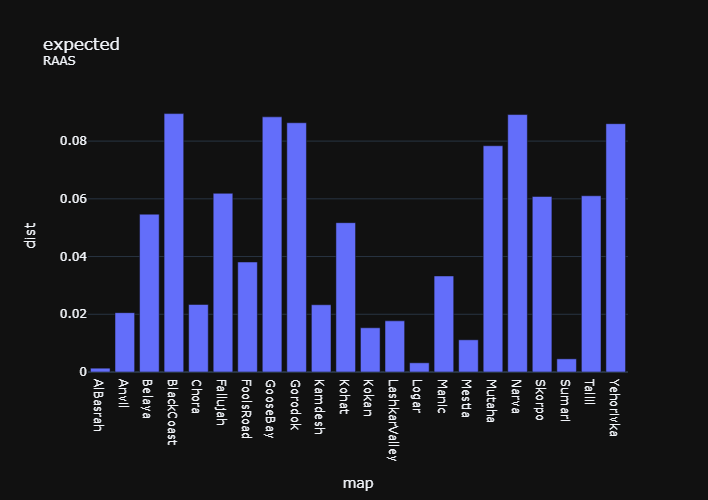
\includegraphics[width=0.7\textwidth]{RAAS_expected.png}
                \caption{erwartete Mapverteilung im Modus RAAS nach den Layervotes vom 19.09.2022}
                \label{fig:expected_mapverteilung_raas}
            \end{figure}

            \begin{figure}[h]
                \centering
                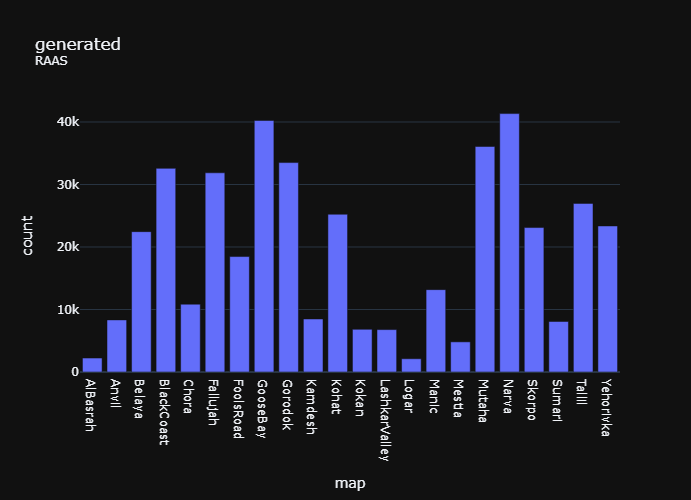
\includegraphics[width=0.7\textwidth]{RAAS_generated.png}
                \caption{generierte Mapverteilung im Modus RAAS nach den Layervotes vom 19.09.2022 (1.Mio. Layer Rota)}
                \label{fig:generated_mapverteilung_raas}
            \end{figure}

            Bei der Betrachtung der Diagramme 
            (Abbildung \ref{fig:expected_mapverteilung_raas} und Abbildung \ref{fig:generated_mapverteilung_raas}) 
            ist zu beachten, dass es sich hier nur um den Modus RAAS handelt.
            Beispielsweise ist die Karte AlBashrah hier deutlich unterrepräsentiert diese ist im Modus Invasion
            nicht der Fall, da die Layervotes dort für AlBashrah deutlich besser ausfallen.
            Zudem lässt sich erkennen, dass die Karte Yehorivka, Blackcoast und Gorodok nicht den angestrebten
            Verteilung erreichen. Dieses Phänomen \ref{s:grenzen_des_systems} näher behandelt.

        \subsubsection{Mode/Modus verteilung}
            Wie bei den Mapverteilungen kann bei den Modusverteilungen die mittlere quadratische Abweichung als
            quantifizierendes Mitteln genommen werden. Bei den Modi ergibt sich eine MSD = $0.04514$.
            Dieser Wert ist für die vorgesehenen Einstellparameter akzeptabel, da Modi die nicht RAAS oder AAS sind
            einen Mindestabstand haben. In diesem Falle ist dieser Abstand 4 Runden.
        \subsubsection{Biom Distanz}
            
        1.0894609482848558
        \subsubsection{Map Wiederholung}
        3
       

        % wie kommt er mit verschiedenen Mapverteilungen klar 
        % Was sind die Einstellungen und warum haben wir so gewählt
    \subsection{Grenzen des Systems}
        \label{s:grenzen_des_systems}
        % unsere limitierendes Feature
        % optimizer warum das ? 
        % warum schlechter wenn Ähnlichkeit des maps und gleichzeitig sehr beliebt
        % warum kann man mit gewissen einstellungen die Rota zu zerstören kann


    \section{Ein Blick in die Glaskugel}
    \usbsection{Diskussion}
        % warum kann man mit gewissen einstellungen die Rota zustören kann
        % warum diese Rota geil ist!
    \subsection{Ausblick}
        % was könnte man noch besser machen 
        % zwei Kugeln setting und Gameplay
        % zweimal die gleich Fraktion und warum schwierig

    \section*{Anhang}



    % \section{Spezifikationen}
    % Im folgenden werden unbekannte Begriffe erklärt und/oder definiert.
    %     \subsection{Allgemeines}
    %         \subsubsection{Spielmodus}
    %             Die aktuell (stand Sep. 2022) auf dem {WLS} Server gespielten Spielmodi sind:\\
    %             \begin{itemize}
    %                 \item RAAS
    %                 \item AAS
    %                 \item Invasion
    %                 \item TC
    %                 \item Insurgency
    %                 \item Destruction
    %                 \item Skirmish\todo{Tanks ?}
    %             \end{itemize}
    %             Die Beschreibung dieser Modi geht über dieses Dokument hinaus.
    %         \subsubsection{Layer}
    %             Ein Layer ist einer Karte und einen Spielmodus zugeordnet.
    %             Pro Runde Squad wird ein Layer gespielt. 
    %         \subsubsection{Maprotation}
    %             Eine Maprotation (kurz Maprota) besteht aus einer Liste von vorgegebene Runden, die gespielt werden sollen.
    %             Jede Runde wird ein Layer gespielt.
    %         \subsubsection{Clustering}
    %             Beschreibt die Wiederholung von Squad Runden mit ähnlichen Eigenschaften in einem kurzem zeitintervall.
    %         \subsection{Attraktive Maprotation}
    %             Eine attraktive Maprota kann durch ihre Rundenverteilung und Rundenreihenfolge beschrieben werden.
    %             Gibt es eine positive Korrelation zwischen Layer-Verteilungen einer Maprota und der Layervote-Verteilung ist der Beliebtheitsgrad höher.
    %             Zudem ist eine Maprota mit kurz aufeinander folgenden, sich stärker unterscheidnenen Maps, beliebter.
    %             \todo{ist ein bisschen aus der Luft gegriffen}
    %     \subsection{Eingabe Parameter}
    %         \subsubsection{Layervote}
    %             Während einer Runde auf einem WLS Server kann das gespielte Layer, von jedem Spieler,
    %             positiv oder negativ bewertet werden.
    %             Diese Stimme einer Person wird Layervote genannt.
    %         \subsubsection{Biom-Bewertung}
    %             Eine Karte in Squad ist einem Platz auf der Welt nachempfunden. 
    %             Für die Einordnung der Karten untereinander werden sie anhand ihrer Eigenschaften bewertet.
    %             Diese Bewertung wird hier Biom-Bewertung genannt.
    %     \subsection{Gruppierung der Spielmodi}
    %             Für eine bessere Übersicht werden hier die Spielmodi Gruppiert.\\
    %             Casual:
    %             \begin{itemize}
    %                 \item RAAS
    %                 \item AAS
    %             \end{itemize}
    %             Intermediates:
    %             \begin{itemize}
    %                 \item TC
    %                 \item Invasion
    %             \end{itemize}
    %             Rest:
    %             \begin{itemize}
    %                 \item Insurgency
    %                 \item Destruction \todo{tanks ?}
    %             \end{itemize}
    
    % \section{Metriken}
    % Um eine erzeuge Maprota Bewerten zu können, muss sie quantifiziert werden. 
    % Dafür werden Metriken definiert welche eine objektive Bewertung, mit gegebenen Daten, zulässt.    



    % \section{Überliegende Struktur}
    % \section{Abhängigkeiten der Generierung}
    % \subsection{Mode}
    % \subsection{Biome}
    % \subsection{Mapgröße}
    % \subsection{Votes}
    % \subsection{Modes pro Map}

    \todo{hier mem colonel einfügen}
    \newpage

    \printbibliography[title=Literaturverzeichnis]
    \addcontentsline{toc}{section}{Literaturverzeichnis}

\end{document}